\documentclass[tikz,border=2pt]{standalone}
\usepackage{amsmath,amssymb}
\usepackage{pgfplots}
\pgfplotsset{compat=1.18}

\begin{document}
% Total variance = average spread within the groups X = 1, 2, 3 (blue) + spread of the group
% means around the overall mean (red).
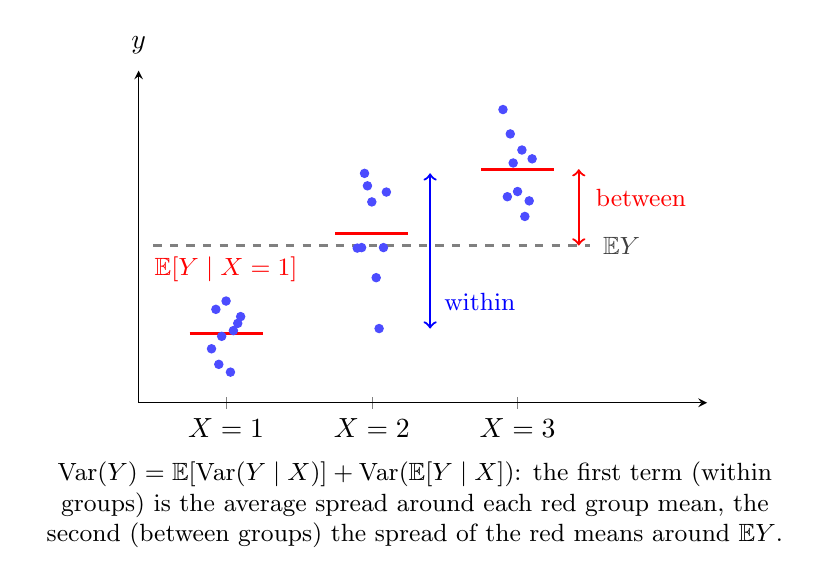
\begin{tikzpicture}
	\begin{axis}[
		axis lines=left, xmin=0.4, xmax=4.3, ymin=0.8, ymax=7.2,
		xtick={1,2,3}, xticklabels={$X=1$,$X=2$,$X=3$}, ytick=\empty,
		ylabel={$y$}, ylabel style={rotate=-90, anchor=south, at={(axis description cs:0,1.02)}},
		width=8.8cm, height=5.8cm, clip=false
		]
		\addplot[only marks, mark=*, mark size=1.5pt, blue!70] coordinates {(0.93,2.60) (1.05,2.19) (0.97,2.08) (1.08,2.33) (0.95,1.54) (1.03,1.39) (1.0,2.76) (0.9,1.84) (1.1,2.46)};
		\addplot[only marks, mark=*, mark size=1.5pt, blue!70] coordinates {(1.93,3.79) (2.05,2.23) (1.97,4.98) (2.08,3.79) (1.95,5.22) (2.03,3.21) (2.0,4.67) (1.9,3.78) (2.1,4.86)};
		\addplot[only marks, mark=*, mark size=1.5pt, blue!70] coordinates {(2.93,4.77) (3.05,4.39) (2.97,5.42) (3.08,4.69) (2.95,5.98) (3.03,5.67) (3.0,4.87) (2.9,6.45) (3.1,5.50)};
		\draw[red, very thick] (axis cs:0.75,2.13) -- (axis cs:1.25,2.13);
		\draw[red, very thick] (axis cs:1.75,4.06) -- (axis cs:2.25,4.06);
		\draw[red, very thick] (axis cs:2.75,5.30) -- (axis cs:3.25,5.30);
		\draw[gray, dashed, thick] (axis cs:0.5,3.83) -- (axis cs:3.5,3.83);
		\node[gray!50!black, anchor=west, font=\small] at (axis cs:3.52,3.83) {$\mathbb{E}Y$};
		\draw[blue, thick, <->] (axis cs:2.4,2.23) -- (axis cs:2.4,5.22);
		\node[blue, anchor=west, font=\small, align=left] at (axis cs:2.43,2.75) {within};
		\draw[red, thick, <->] (axis cs:3.42,3.83) -- (axis cs:3.42,5.30);
		\node[red, anchor=west, font=\small, align=left] at (axis cs:3.47,4.75) {between};
		\node[red, anchor=south, font=\small] at (axis cs:1,2.95) {$\mathbb{E}[Y\mid X=1]$};
	\end{axis}
	\node[anchor=north, font=\small, align=flush center, text width=9.6cm] at ([yshift=-2pt]current axis.outer south) {$\operatorname{Var}(Y)=\mathbb{E}[\operatorname{Var}(Y\mid X)]+\operatorname{Var}(\mathbb{E}[Y\mid X])$: the first term (within groups) is the average spread around each red group mean, the second (between groups) the spread of the red means around $\mathbb{E}Y$.};
\end{tikzpicture}
\end{document}
